


%% Canadian Association of Physicists
%%----------------------------------------


%% CAP High School Prize Examinations
%%----------------------------------------


%% CAP Exam 1997 Part A: Multiple Choice Questions
%%--------------------------------------------------
\element{cap}{
\begin{question}{CAP-A-1997-q01}
    Two astronauts, each of mass \SI{75}{\kilo\gram}, are floating next to each other in space,
        outside the space shuttle.
    One of the them pushes the other through a distance of \SI{1}{\meter}
        (an arm's length) with a force of \SI{300}{\newton}.
    What is the final relative velocity of the two?
    \begin{multicols}{2}
    \begin{choices}
        \wrongchoice{\SI{2.0}{\meter\per\second}}
        \wrongchoice{\SI{2.83}{\meter\per\second}}
        \wrongchoice{\SI{4.0}{\meter\per\second}}
        \wrongchoice{\SI{16.0}{\meter\per\second}}
    \end{choices}
    \end{multicols}
\end{question}
}

\element{cap}{
\begin{question}{CAP-A-1997-q02}
    Twelve identical resistors (each of resistance $R$) are placed along the 12 edges of a cube.
    What is the effective resistance between opposite corners of the cube?
    \begin{multicols}{2}
    \begin{choices}
        \wrongchoice{$\dfrac{2R}{3}$}
        \wrongchoice{$\dfrac{5R}{3}$}
        \wrongchoice{$R$}
        \wrongchoice{$12 R$}
    \end{choices}
    \end{multicols}
\end{question}
}


%% CAP Exam 1996 Part A: Multiple Choice Questions
%%--------------------------------------------------
\element{cap}{
\begin{question}{CAP-A-1996-q01}
    A toy for firing a ball vertically consists of a vertical spring which is compressed by \SI{0.10}{\meter}.
    A force of \SI{10.0}{\newton} is needed to hold the spring at that compression.
    If a ball of mass \SI{0.050}{\kilo\gram} is placed on the compressed spring and the spring is released,
        the ball will reach a height (above its initial position) of:
    \begin{multicols}{2}
    \begin{choices}
      \correctchoice{\SI{1.0}{\meter}}
        \wrongchoice{\SI{1.2}{\meter}}
        \wrongchoice{\SI{1.4}{\meter}}
        \wrongchoice{\SI{1.6}{\meter}}
    \end{choices}
    \end{multicols}
\end{question}
}

\element{cap}{
\begin{question}{CAP-A-1996-q02}
    A rescue plane is flying horizontally with a speed of \SI{30}{\meter\per\second} and at an altitude of \SI{125}{\meter} above the sea when it drops a warning flare.
    Neglecting air resistance and assuming that the plane does not change its course,
        speed or altitude, how far from the plane is the flare when it hits the water?
    \begin{multicols}{2}
    \begin{choices}
        \wrongchoice{\SI{146}{\meter}}
        \wrongchoice{\SI{195}{\meter}}
      \correctchoice{\SI{125}{\meter}}
        \wrongchoice{\SI{150}{\meter}}
    \end{choices}
    \end{multicols}
\end{question}
}

\element{cap}{
\begin{question}{CAP-A-1996-q03}
    A loudspeaker is placed over the open end of a pipe.
    By changing the frequency of the sound from the speaker,
        it is found that the pipe has resonances at \SI{700}{\hertz} and \SI{900}{\hertz} but not \SI{800}{\hertz}.
    This means that:
    \begin{choices}
      \correctchoice{The pipe is closed at one end and the fundamental is \SI{100}{\hertz}}
        \wrongchoice{The pipe is closed at one end and the fundamental is \SI{200}{\hertz}}
        \wrongchoice{The pipe is open at both ends and the fundamental is \SI{100}{\hertz}}
        \wrongchoice{The pipe is open at both ends and the fundamental is \SI{200}{\hertz}}
    \end{choices}
\end{question}
}

\element{cap}{
\begin{question}{CAP-A-1996-q04}
    In a television tube,
        electrons are accelerated from rest through a potential difference of \SI{1600}{\volt}.
    What is the speed of the electrons after this acceleration?
    \begin{multicols}{2}
    \begin{choices}
        \wrongchoice{\SI{16 000}{\kilo\meter\per\second}}
        \wrongchoice{\SI{20 000}{\kilo\meter\per\second}}
      \correctchoice{\SI{24 000}{\kilo\meter\per\second}}
        \wrongchoice{\SI{28 000}{\kilo\meter\per\second}}
    \end{choices}
    \end{multicols}
\end{question}
}

\element{cap}{
\begin{question}{CAP-A-1996-q05}
    The electron-volt is a measure of:
    \begin{choices}
        \wrongchoice{charge}
        \wrongchoice{current}
        \wrongchoice{electric field strength}
      \correctchoice{energy}
    \end{choices}
\end{question}
}

\element{cap}{
\begin{question}{CAP-A-1996-q06}
    A current of \SI{5}{\ampere} passes along a wire of length \SI{1.0}{\meter}.
    The wire is at right angles to a uniform magnetic field of strength \SI{0.15}{\tesla}.
    The force on the wire is:
    \begin{multicols}{2}
    \begin{choices}
        \wrongchoice{zero}
      \correctchoice{\SI{0.75}{\newton}}
        \wrongchoice{\SI{33}{\newton}}
        \wrongchoice{\SI{0.03}{\newton}}
    \end{choices}
    \end{multicols}
\end{question}
}

\element{cap}{
\begin{question}{CAP-A-1996-q07}
    An \SI{8}{\micro\farad} capacitor is charged to a potential of \SI{120}{\volt}.
    How much work was required to do this?
    \begin{multicols}{2}
    \begin{choices}
        \wrongchoice{\SI{2.7e-12}{\joule}}
        \wrongchoice{\SI{1.2e-1}{\joule}}
        \wrongchoice{\SI{9.6e-4}{\joule}}
      \correctchoice{\SI{5.8e-2}{\joule}}
    \end{choices}
    \end{multicols}
\end{question}
}

\element{cap}{
\begin{question}{CAP-A-1996-q08}
    A flashlight is operated on four batteries placed in series.
    Each battery has an internal resistance $r$.
    If one of the batteries is accidently placed the wrong way around,
        the total interal resistance of the four cells will not be:
    \begin{multicols}{2}
    \begin{choices}
        \wrongchoice{$\dfrac{r}{4}$}
        \wrongchoice{$3 r$}
        \wrongchoice{$\dfrac{r}{5}$}
      \correctchoice{$4 r$}
    \end{choices}
    \end{multicols}
\end{question}
}

\element{cap}{
\begin{question}{CAP-A-1996-q09}
    A ray of light is passing from air into glass.
    If the angle of incidence,
        with respect to the normal to the interface,
        is increased:
    \begin{choices}
        \wrongchoice{Total internal reflection will occur when the angle of incidence equals the critical angle.}
        \wrongchoice{Total internal reflection will occur when the angle of incidence is less than the critical angle.}
        \wrongchoice{Total internal reflection will occur when the angle of incidence is greater than the critical angle.}
      \correctchoice{The refractive angle will increase but there will be no total internal reflection.}
    \end{choices}
\end{question}
}

\element{cap}{
\begin{question}{CAP-A-1996-q10}
    A mass of \SI{20}{\gram} is hung from the end of a light vertical spring and is set oscillating with an amplitude of \SI{10}{\centi\meter}.
    Its total energy is found to be \SI{4}{\joule}.
    If the mass is now replaced with a mass of \SI{40}{\gram} and it is again set oscillating with an amplitude of \SI{10}{\centi\meter},
        its total energy is now:
    \begin{multicols}{2}
    \begin{choices}
        \wrongchoice{\SI{2}{\joule}}
      \correctchoice{\SI{4}{\joule}}
        \wrongchoice{\SI{5.6}{\joule}}
        \wrongchoice{\SI{8}{\joule}}
    \end{choices}
    \end{multicols}
\end{question}
}

\element{cap}{
\begin{question}{CAP-A-1996-q11}
    A \SI{65}{\kilo\gram} girl, riding an elevator,
        weights herself by standing on a scale.
    What is the reading of the scale is the elevator is accelerating downwards at \SI{2}{\meter\per\second\squared}?
    \begin{multicols}{2}
    \begin{choices}
        \wrongchoice{\SI{65.0}{\kilo\gram}}
        \wrongchoice{\SI{0}{\kilo\gram}}
      \correctchoice{\SI{51.7}{\kilo\gram}}
        \wrongchoice{\SI{78.3}{\kilo\gram}}
    \end{choices}
    \end{multicols}
\end{question}
}

\element{cap}{
\begin{question}{CAP-A-1996-q12}
    A highway curve of radius \SI{30}{\meter} is banked so that a car travelling at \SI{40}{\kilo\meter\per\hour} can travel around it without slipping even if there is no friction between the car's tires and the road surface.
    Without friction,
        a car travelling faster than this will slide up the curve,
        while a car travelling slower will slide down the curve.
    Find the angle of elevation of the banked highway curve.
    \begin{multicols}{2}
    \begin{choices}
        \wrongchoice{\ang{67}}
      \correctchoice{\ang{23}}
        \wrongchoice{\ang{45}}
        \wrongchoice{\ang{90}}
    \end{choices}
    \end{multicols}
\end{question}
}

\element{cap}{
\begin{question}{CAP-A-1996-q13}
    A ball is thrown upwards into the air rising to a height $h$.
    Accounting for the ``real life'' conditions of air resistance,
        the time $t_1$ that the ball takes to rise to its maximum height and time $t_2$ that is takes to fall back down to its initial position obey:
    \begin{multicols}{2}
    \begin{choices}
        \wrongchoice{$t_1 = t_2$}
      \correctchoice{$t_1 < t_2$}
        \wrongchoice{$t_1 > t_2$}
        \wrongchoice{$t_1 + t_2 = \sqrt{\dfrac{8h}{g}}$}
    \end{choices}
    \end{multicols}
\end{question}
}

\element{cap}{
\begin{question}{CAP-A-1996-q14}
    An airplane flies northwards from town $A$ to town $B$ and then back again.
    There is a steady wind blowing towards the north so that for the first stage of the trip,
        the airplane is flying in the same direction as the wind and for the return half of the journey,
        the airplane is flying directly into the wind.
    The total trip time $T_w$, as compared to the total trip time in the absence of any wind $T_0$, obeys:
    \begin{multicols}{2}
    \begin{choices}
        \wrongchoice{$T_w = T_0$}
      \correctchoice{$T_w > T_0$}
        \wrongchoice{$T_w < T_0$}
        \wrongchoice{$T_w = 2 T_0$}
    \end{choices}
    \end{multicols}
\end{question}
}

\element{cap}{
\begin{question}{CAP-A-1996-q15}
    The space shuttle moves in a circular orbit about the earth at a constant speed.
    To change the orbit radius,
        the crew temporariliy activates the main engine which accelerates the space shuttle in the direction of its motion.
    After the main engine is switched off again,
        the shuttle will be in an elliptical orbit with:
    \begin{choices}
      \correctchoice{a larger average radius and a lower average speed.}
        \wrongchoice{a larger average radius and a higher average speed.}
        \wrongchoice{a smaller average radius and a lower average speed.}
        \wrongchoice{a smaller average radius and a higher average speed.}
    \end{choices}
\end{question}
}

\element{cap}{
\begin{question}{CAP-A-1996-q16}
    Which of the following expressions has the correct units to represent the radius of a hydrogen atom in its ground state?
    (only one expression is correct)
    \begin{multicols}{2}
    \begin{choices}
      \correctchoice{$\dfrac{\varepsilon_0 h^2}{\pi m_e e^2}$}
        \wrongchoice{$\dfrac{h^2 m_e e^2}{4\pi \varepsilon_0}$}
        \wrongchoice{$\dfrac{m_e c^2}{h^2 e^4}$}
        \wrongchoice{$\dfrac{e^4 m_e}{8 \varepsilon_0^2 h^2}$}
    \end{choices}
    \end{multicols}
\end{question}
}

\element{cap}{
\begin{question}{CAP-A-1996-q17}
    If the electric field is zero within some region of space,
        the electric potential within that region:
    \begin{choices}
        \wrongchoice{must be zero.}
        \wrongchoice{must be positive.}
        \wrongchoice{must be negative.}
      \correctchoice{must be a constant value.}
    \end{choices}
\end{question}
}

\element{cap}{
\begin{question}{CAP-A-1996-q18}
    In comparing properties of visible light waves to microwaves,
        which of the following statements is \emph{false}?
    \begin{choices}
      \correctchoice{Visible light waves travel at the same speed in glass as do microwaves.}
        \wrongchoice{Visible light waves have a higher frequency in glass than do microwaves.}
        \wrongchoice{Visible light waves travel at the same speed in vacuum as do microwaves.}
        \wrongchoice{Both visible light waves and microwaves can be refracted by glass.}
    \end{choices}
\end{question}
}

\element{cap}{
\begin{question}{CAP-A-1996-q19}
    A boy sits at the top of a hemispherical mound of ice of radius $r$.
    He begins to slide (from rest) downwards without friction.
    At what height above the ground does he leave contact with the ice?
    \begin{choices}
        \wrongchoice{The boy does not leave contact with the ice.}
        \wrongchoice{$\dfrac{r}{3}$}
        \wrongchoice{$\dfrac{r}{2}$}
      \correctchoice{$\dfrac{2r}{3}$}
    \end{choices}
\end{question}
}

\element{cap}{
\begin{question}{CAP-A-1996-q20}
    A rocket for mining the asteroid belt is designed like a large scoop.
    It is approaching asteroids at a velocity of \SI{e4}{\meter\per\second}.
    The asteroids are much smaller than the rocket.
    If the rocket scoops asteroids at the rate of \SI{100}{\kilo\gram\per\second},
        what thrust (force) must the rocket's engines provide in order for the rocket to maintain a constant velocity?
    Ignore any variation in the rocket's mass due to the burning of fuel.
    \begin{multicols}{2}
    \begin{choices}
        \wrongchoice{\SI{e3}{\newton}}
      \correctchoice{\SI{e5}{\newton}}
        \wrongchoice{\SI{e9}{\newton}}
        \wrongchoice{\SI{e12}{\newton}}
    \end{choices}
    \end{multicols}
\end{question}
}

\element{cap}{
\begin{question}{CAP-A-1996-q21}
    The sensitivity of the human ear is greatest near \SI{3000}{\hertz}.
    This result is best explained by the fact that:
    \begin{choices}
      \correctchoice{the ear canal is a resonant cavity with a fundamental frequency near \SI{3000}{\hertz}.}
        \wrongchoice{at a frequency of \SI{3000}{\hertz} the wavelength of sound is approximately the distance between the ears.}
        \wrongchoice{\SI{3000}{\hertz} is the frequency at which the skull resonates.}
        \wrongchoice{none of the provided statements explain the result.}
    \end{choices}
\end{question}
}

\element{cap}{
\begin{question}{CAP-A-1996-q22}
    A long piece of rubber is wider than it is thick.
    When it is stretched in length by some amount:
    NOTE: assume that length, width and thickness are perpendicular
    \begin{choices}
        \wrongchoice{its thickness decreases but its width increases.}
        \wrongchoice{its thickness decreases but its width remains the same.}
        \wrongchoice{its thickness increases but its width decreases.}
      \correctchoice{both its thickness and width decreases.}
    \end{choices}
\end{question}
}

\element{cap}{
\begin{question}{CAP-A-1996-q23}
    A new medical procedure to cure near-sightedness involves changing the shape of the eye's lens using a precisely controlled laser beam.
    A near-sighted eye cannot focus clearly on distant objects.
    To improve the vision of the patient, we must:
    \begin{choices}
        \wrongchoice{uniformly decrease the thickness of the lens.}
        \wrongchoice{uniformly increase the thickness of the lens.}
      \correctchoice{make the middle of the lens thinner.}
        \wrongchoice{make the outer rim of the lens thinner.}
    \end{choices}
\end{question}
}

\element{cap}{
\begin{question}{CAP-A-1996-q24}
    A proton travels in a circular orbit of radius \SI{1}{\centi\meter} in a magnetic field of strength \SI{0.5}{\tesla}.
    The kinetic energy of the proton is:
    \begin{multicols}{2}
    \begin{choices}
        \wrongchoice{\SI{3.35e-27}{\joule}}
        \wrongchoice{\SI{1.67e-27}{\joule}}
        \wrongchoice{\SI{3.83e-16}{\joule}}
      \correctchoice{\SI{1.91e-16}{\joule}}
    \end{choices}
    \end{multicols}
\end{question}
}

\element{cap}{
\begin{question}{CAP-A-1996-q25}
    A metal rod \SI{30}{\centi\meter} long moves at \SI{8}{\meter\per\second} in a plane perpendicular to a magnetic field of \SI{0.05}{\tesla}.
    The velocity of the rod is in a direction perpendicular to its length.
    The potential difference between the ends of the rod is:
    \begin{multicols}{2}
    \begin{choices}
        \wrongchoice{\SI{48}{\volt}}
        \wrongchoice{\SI{6.40e-20}{\volt}}
      \correctchoice{\SI{120}{\milli\volt}}
        \wrongchoice{A potential difference will not be induced in this case.}
    \end{choices}
    \end{multicols}
\end{question}
}



%% CAP Exam 1995 Part A: Multiple Choice Questions
%%--------------------------------------------------
\element{cap}{
\begin{question}{CAP-A-1995-q01}
    A salvage ship tries to raise a sunken miniature submarine from the bottom of Lake Superior.
    The submarine and its contents have a mass of \SI{72 000}{\kilo\gram} and a volume of \SI{18.9}{\meter\cubed}.
    What upwards force must be applied to raise the submarine?
    The density of water is \SI{1000}{\kilo\gram\per\meter\cubed}?
    \begin{multicols}{2}
    \begin{choices}
        \wrongchoice{\SI{1.8e5}{\newton}}
        \wrongchoice{\SI{2.0e5}{\newton}}
        \wrongchoice{\SI{4.8e5}{\newton}}
      \correctchoice{\SI{5.2e5}{\newton}}
    \end{choices}
    \end{multicols}
\end{question}
}

\element{cap}{
\begin{question}{CAP-A-1995-q02}
    A little girl is playing with a toy pendulum while riding in an elevator.
    Being an astute and educated young lass,
        she notes that the period of the pendulum is $T=\SI{0.5}{\second}$.
    Suddenly the cabels supporting the elevator break and all of the safety features fail simulataneously.
    The elevator plunges into free fall.
    The yound girl is astonished to discover that the pendulum has,
    \begin{choices}
        \wrongchoice{continued oscillating with a period of \SI{0.5}{\second}.}
      \correctchoice{stopped oscillating entirely.}
        \wrongchoice{decreased its rate of oscillation to have a greater period.}
        \wrongchoice{decreased its rate of oscillation to have a lesser period.}
    \end{choices}
\end{question}
}

\element{cap}{
\begin{question}{CAP-A-1995-q03}
    Two identical spring loaded, toy guns shoot projectiles straight upwards.
    The projectile in gun $B$ has twice the mass as that in gun $A$.
    The projectile launched by gun $A$ reaches a height $H$.
    Ignoring air resistance, the projectile launched by gun $B$ would reach a height of:
    \begin{multicols}{2}
    \begin{choices}
        \wrongchoice{$\dfrac{H}{4}$}
      \correctchoice{$\dfrac{H}{2}$}
        \wrongchoice{$\dfrac{H}{\sqrt{2}}$}
        \wrongchoice{$H$}
    \end{choices}
    \end{multicols}
\end{question}
}

\element{cap}{
\begin{question}{CAP-A-1995-q04}
    An athlete of mass \SI{75}{\kilo\gram} runs at \SI{10}{\meter\per\second}.
    What is his kinetic energy?
    \begin{multicols}{2}
    \begin{choices}
      \correctchoice{\SI{3750}{\joule}}
        \wrongchoice{\SI{7500}{\joule}}
        \wrongchoice{\SI{375}{\joule}}
        \wrongchoice{\SI{750}{\joule}}
    \end{choices}
    \end{multicols}
\end{question}
}

\element{cap}{
\begin{question}{CAP-A-1995-q05}
    The moon is about 60 earth radii from the center of the earth and completes one orbit in about 28 days.
    Assuming that the moon executes a circular orbit about the center of the earth,
        the acceleration of the moon (in units of $g$, the acceleration due to gravity at the earth's surface) is closest to,
    \begin{multicols}{2}
    \begin{choices}
        \wrongchoice{$\dfrac{g}{30}$}
        \wrongchoice{$\dfrac{g}{60}$}
      \correctchoice{$\dfrac{g}{3600}$}
        \wrongchoice{$g$}
    \end{choices}
    \end{multicols}
\end{question}
}

\element{cap}{
\begin{question}{CAP-A-1995-q06}
    A survey crew sights the top of a radio tower with a small telescope.
    The angle that the telescope makes with the horizontal is measured to be \ang{53}.
    The crew moves the telescope \SI{25}{\meter} closer to teh base of the tower and repeats the process.
    The new angle that the telescope makes with the horizontal is \ang{60}.
    What is the height of the tower assuming that the base of the tower is on the same level as the area where the telescope measurements were made?
    \begin{multicols}{2}
    \begin{choices}
        \wrongchoice{\SI{33}{\meter}}
        \wrongchoice{\SI{43}{\meter}}
      \correctchoice{\SI{142}{\meter}}
        \wrongchoice{\SI{286}{\meter}}
    \end{choices}
    \end{multicols}
\end{question}
}

\element{cap}{
\begin{question}{CAP-A-1995-q07}
    Which of the followig is \emph{not} true for electromagnetic waves:
    \begin{choices}
        \wrongchoice{they consist of oscillating electric and magnetic fields.}
        \wrongchoice{they travel at different speeds in air depending on their frequency.}
        \wrongchoice{they transport energy.}
      \correctchoice{they have no momentum.}
    \end{choices}
\end{question}
}

\element{cap}{
\begin{question}{CAP-A-1995-q08}
    Two long parallel wires are placed side-by-side on a level table.
    The two wires carry equal currents in the same direction.
    Which of the following is true of the magnetic forces exerted on each wire by the other?
    \begin{choices}
        \wrongchoice{One wire experiences a force upwards while the other experiences a downwards force.}
        \wrongchoice{Both wires experience an upwards force.}
      \correctchoice{The two wires are attracted to one another.}
        \wrongchoice{The two wires repel one another.}
    \end{choices}
\end{question}
}

\element{cap}{
\begin{question}{CAP-A-1995-q09}
    A piano tuner uses a tuning fork which oscillates with a frequency of \SI{440}{\hertz} (middle A).
    Middle A on a piano is out of tune,
        producing a note of frequency $f$.
    The piano note and the tuning fork are heard to beat with a frequency of \SI{3}{\hertz}.
    When the tension in the piano string is decreased,
        the beat frequency also decreases.
    The out-of-tune frequency $f$ must have been,
    \begin{multicols}{2}
    \begin{choices}
        \wrongchoice{\SI{446}{\hertz}}
      \correctchoice{\SI{443}{\hertz}}
        \wrongchoice{\SI{437}{\hertz}}
        \wrongchoice{\SI{434}{\hertz}}
    \end{choices}
    \end{multicols}
\end{question}
}

\element{cap}{
\begin{question}{CAP-A-1995-q10}
    Sudbury's Creighton mine is one of the deepest in the world (\SI{2.07}{\kilo\meter}).
    In this mine the conditions as compare to those at the surface are,
    \begin{choices}
        \wrongchoice{lower air pressure, higher acceleration due to gravity.}
      \correctchoice{higher air pressure, lower acceleration due to gravity.}
        \wrongchoice{higher air pressure, higher acceleration due to gravity.}
        \wrongchoice{lower air pressure, lower acceleration due to gravity.}
    \end{choices}
\end{question}
}

\element{cap}{
\begin{question}{CAP-A-1995-q11}
    A parallel network of resistors consists of a \SI{1}{\ohm} resistor placed in parallel with a \SI{2}{\ohm} resistor.
    This combination is,
        in turn, placed in parallel with a \SI{4}{\ohm} resistor.
    Further \SI{8}{\ohm}, \SI{16}{\ohm}, \SI{32}{\ohm} \ldots resistors are placed in parallel with the network one by one.
    To what value does equivalent resistance of the network converte upon?
    \begin{multicols}{2}
    \begin{choices}
      \correctchoice{\SI{0.5}{\hertz}}
        \wrongchoice{\SI{2.0}{\hertz}}
        \wrongchoice{\SI{0.0}{\hertz}}
        \wrongchoice{Does not converge to a finite value.}
    \end{choices}
    \end{multicols}
\end{question}
}

\element{cap}{
\begin{question}{CAP-A-1995-q12}
    A simple machine has a bob of mass \SI{2}{\kilo\gram} hanging on a cord of length \SI{1}{\meter}.
    Suppose the pendulum is raised until it is horizontal (an angular displacement of \ang{90}) and then released.
    What is the speed of the bob at the bottom of its swing?
    \begin{multicols}{2}
    \begin{choices}
        \wrongchoice{\SI{9.91}{\meter\per\second}}
        \wrongchoice{\SI{19.6}{\meter\per\second}}
        \wrongchoice{\SI{3.13}{\meter\per\second}}
      \correctchoice{\SI{4.43}{\meter\per\second}}
    \end{choices}
    \end{multicols}
\end{question}
}

\element{cap}{
\begin{question}{CAP-A-1995-q13}
    An organ pipe of length $L$ is open at one end and closed at the other.
    What are the wavelength of the three lowest frequencies that can be produced with this pipe?
    \begin{multicols}{2}
    \begin{choices}
        \wrongchoice{$4L$, $2L$, $L$}
        \wrongchoice{$2L$, $L$, $L/2$}
        \wrongchoice{$2L$, $L$, $2L/3$}
      \correctchoice{$4L$, $4L/3$, $4L/5$}
    \end{choices}
    \end{multicols}
\end{question}
}

\element{cap}{
\begin{question}{CAP-A-1995-q14}
    A satellite is in orbit at an altitue of one earth radius.
    What is the orbital speed of this satellite?
    \begin{multicols}{2}
    \begin{choices}
        \wrongchoice{\SI{1.56e7}{\meter\per\second}}
        \wrongchoice{\SI{3.95e3}{\meter\per\second}}
        \wrongchoice{\SI{9.91e3}{\meter\per\second}}
      \correctchoice{\SI{5.59e3}{\meter\per\second}}
    \end{choices}
    \end{multicols}
\end{question}
}

\element{cap}{
\begin{question}{CAP-A-1995-q15}
    A stead non-turbulent stream of water comes out of a tap and falls verticall downward.
    As it does so,
        the diameter of the stream appears to get smaller.
    What is the primary reason?
    \begin{choices}
        \wrongchoice{The water's surface tension constricts the stream.}
        \wrongchoice{Air pressure, which decreases with altitude, squeezes the stream}
      \correctchoice{The water is accelerating under gravity and so the stream must get thinner as the flow rate (velocity times cross-sectional area) must be constant.}
        \wrongchoice{The flow does not constrict; it is an optical illusion.}
    \end{choices}
\end{question}
}

\element{cap}{
\begin{question}{CAP-A-1995-q16}
    A roller coaster car is on a track that forms a circular loop,
        of radius $R$, in the vertical plane.
    If the car is to maintain contact with the track at the top of the loop
        (generally considered to be a good thing),
        what is the minimum speed that the car must have at the bottom of the loop.
    Ignore air resistance and rolling friction.
    \begin{multicols}{2}
    \begin{choices}
        \wrongchoice{$\sqrt{2gR}$}
        \wrongchoice{$\sqrt{3gR}$}
        \wrongchoice{$\sqrt{4gR}$}
      \correctchoice{$\sqrt{5gR}$}
    \end{choices}
    \end{multicols}
\end{question}
}

\element{cap}{
\begin{question}{CAP-A-1995-q17}
    An object is placed \SI{30}{\centi\meter} in front of a thin,
        spherical lens.
    An upright image, twice the size of the object,
        is formed by the lens.
    Which of the following attributes best describes the lens.
    \begin{choices}
        \wrongchoice{diverging, focal length \SI{20}{\centi\meter}}
        \wrongchoice{convergin, focal length \SI{20}{\centi\meter}}
        \wrongchoice{diverging, focal length \SI{60}{\centi\meter}}
      \correctchoice{convergin, focal length \SI{60}{\centi\meter}}
    \end{choices}
\end{question}
}

\element{cap}{
\begin{question}{CAP-A-1995-q18}
    A point charge $+Q$ is placed at the centroid of an equilateral triangle.
    When a second charge $+Q$ is placed at a vertex of the triangle,
        the magnitude of the electrostatic force on the central charge is \SI{4}{\newton}.
    What is the magnitude of the net force on the central charge when a third charge $+Q$ is placed at another vertex of the triangle?
    \begin{multicols}{2}
    \begin{choices}
        \wrongchoice{zero}
      \correctchoice{\SI{4}{\newton}}
        \wrongchoice{\SI[parse-numbers=false]{4\sqrt{2}}{\newton}}
        \wrongchoice{\SI{8}{\newton}}
    \end{choices}
    \end{multicols}
\end{question}
}

\element{cap}{
\begin{question}{CAP-A-1995-q19}
    Greenhouse ``warming'' is caused by an atmosphere which is,
    \begin{choices}
      \correctchoice{transparent to visible light but opaque to I.R. light.}
        \wrongchoice{transparent to both visible and I.R. light.}
        \wrongchoice{opaque to both visible and I.R. light.}
        \wrongchoice{warming due to the hot air from the world's increasing population.}
    \end{choices}
\end{question}
}

\element{cap}{
\begin{question}{CAP-A-1995-q20}
    A particle of mass $m$ and charge $q$ is accelerated through a potential difference $V$ to a velocity $\vec{v}$ towards the south.
    The particle enters a region with both a magnetic field $\vec{B}$ (pointing eastward) and electric field $\vec{E}$ (pointing down).
    The particle travels at constant velocity through this region.
    The potential difference $V$ must satisify,
    \begin{multicols}{2}
    \begin{choices}
      \correctchoice{$V = \dfrac{mE^2}{2qB^2}$}
        \wrongchoice{$V = \dfrac{2mE}{qB}$}
        \wrongchoice{$V = \dfrac{E}{qB}$}
        \wrongchoice{It is not possible for the particle to be undeflected by these fields.}
    \end{choices}
    \end{multicols}
\end{question}
}

\element{cap}{
\begin{question}{CAP-A-1995-q21}
    A space craft orbiting the moon with an orbital radius of \SI{e6}{\meter} has an orbital period of \SI{45}{\minute}.
    When it drops down to a lower radius of radius \SI{e5}{\meter},
        its period has become,
    \begin{multicols}{2}
    \begin{choices}
        \wrongchoice{\SI{36}{\minute}}
      \correctchoice{\SI{85}{\minute}}
        \wrongchoice{\SI{54}{\minute}}
        \wrongchoice{Need to know the mass of the moon for this problem.}
    \end{choices}
    \end{multicols}
\end{question}
}

\element{cap}{
\begin{question}{CAP-A-1995-q22}
    A simple pendulum is made from a \SI{2}{\kilo\gram} block of wood suspended from a light cord of length \SI{1}{\meter}.
    When the pendulum is hanging in such a way that it is stationary and vertical,
        a bullet is shot horizontally into the block of wood where it sticks.
    The bullet has a mass of \SI{e-2}{\kilo\gram} and has a speed of \SI{500}{\meter\per\second} just before its head-on collision with the block.
    The pendulum will swing to a maximum angle with the vertical of,
    \begin{multicols}{2}
    \begin{choices}
        \wrongchoice{\ang{71.3}}
        \wrongchoice{\ang{23.4}}
        \wrongchoice{\ang{35.7}}
      \correctchoice{\ang{46.8}}
    \end{choices}
    \end{multicols}
\end{question}
}

\element{cap}{
\begin{question}{CAP-A-1995-q23}
    Electronic components are testest for durability by subjecting them to high accelerations.
    This is achieved by placing them on a platform attached to a vertically hanging spring.
    The platform (and the component being tested) oscillate up and down with a frequency of \SI{10}{\hertz} when the spring is stretched by \SI{10}{\centi\meter} and released.
    What is the maximum acceleration experienced by the elctronic component?
    \begin{multicols}{2}
    \begin{choices}
        \wrongchoice{\SI{10.0}{\meter\per\second\squared}}
        \wrongchoice{\SI{2.00}{\meter\per\second\squared}}
      \correctchoice{\SI{395}{\meter\per\second\squared}}
        \wrongchoice{\SI{158}{\meter\per\second\squared}}
    \end{choices}
    \end{multicols}
\end{question}
}

\element{cap}{
\begin{question}{CAP-A-1995-q24}
    A real battery can be considered to be an ideal battery of potential $\epsilon$ in series with an internal resistor $r$.
    Suppose that the battery is connected to a single ``load'' resistance $R$.
    For what value of $R$ will the power dissipated by the load be a maximum?
    \begin{multicols}{2}
    \begin{choices}
      \correctchoice{$r$}
        \wrongchoice{$\dfrac{r}{2}$}
        \wrongchoice{$2r$}
        \wrongchoice{$10 r$}
    \end{choices}
    \end{multicols}
\end{question}
}

\element{cap}{
\begin{question}{CAP-A-1995-q25}
    Two trucks pull on either end of a rope,
        each with a force of \SI{10 000}{\newton}.
    In the center of the rope, a ball of mass \SI{20}{\kilo\gram} is hanging.
    \begin{center}
    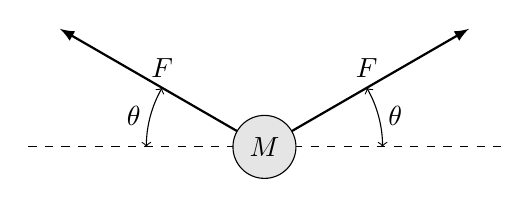
\begin{tikzpicture}
        %% Forces
        \draw[thick,-latex] (0,0) -- (30:3) node[pos=0.5,anchor=south] {$F$};
        \draw[thick,-latex] (0,0) -- (150:3) node[pos=0.5,anchor=south] {$F$};
        %% angle
        \draw[dashed] (-3,0) -- (+3,0);
        \draw[<->] (+1.5,0) arc (0:30:1.5) node[pos=0.5,anchor=west] {$\theta$};
        \draw[<->] (-1.5,0) arc (180:150:1.5) node[pos=0.5,anchor=east] {$\theta$};
        %% Ball
        \node[draw,circle,minimum size=0.8cm,fill=white!90!black,anchor=center] at (0,0) {$M$};
    \end{tikzpicture}
    \end{center}
    The angle $\theta$ that the rope makes with the horizontal is,
    \begin{multicols}{2}
    \begin{choices}
        \wrongchoice{\ang{56}}
        \wrongchoice{\ang{5.6}}
      \correctchoice{\ang{0.56}}
        \wrongchoice{\ang{0}; the rope will obviously be horizontal in this situation.}
    \end{choices}
    \end{multicols}
\end{question}
}


%% CAP Exam 1994 Part A: Multiple Choice Questions
%%--------------------------------------------------
\element{cap}{
\begin{question}{CAP-A-1994-q01}
    It was once proposed to use a \SI{2}{\kilo\meter} vertical Sudbury mine shaft for microgravity experiments in a vacuum.
    How much time would scientists have to do an experiment during one drop?
    \begin{multicols}{2}
    \begin{choices}
      \correctchoice{\SI{20}{\second}}
        \wrongchoice{\SI{63}{\second}}
        \wrongchoice{\SI{0.64}{\second}}
        \wrongchoice{\SI{198}{\second}}
    \end{choices}
    \end{multicols}
\end{question}
}

\element{cap}{
\begin{question}{CAP-A-1994-q02}
    If the moon were twice as massive as it is now,
        and it stayed at the same orbital radius about the earth as it has now,
        its new orbital period (in terms of its current orbital period $T$) would be:
    \begin{multicols}{2}
    \begin{choices}
      \correctchoice{$T$}
        \wrongchoice{$\dfrac{T}{2}$}
        \wrongchoice{$\dfrac{T}{4}$}
        \wrongchoice{$2T$}
    \end{choices}
    \end{multicols}
\end{question}
}

\element{cap}{
\begin{question}{CAP-A-1994-q03}
    In the following circuit composed of identical CAP-Acitors,
    \begin{center}
    \begin{circuitikz}
        %% NOTE: TODO: draw
    \end{circuitikz}
    \end{center}
        across which terminals would you connect a battery in order for all the CAP-Acitors to charge up.
    \begin{multicols}{2}
    \begin{choices}
        \wrongchoice{$AB$}
        \wrongchoice{$AC$}
      \correctchoice{$BD$}
        \wrongchoice{none of the provided}
    \end{choices}
    \end{multicols}
\end{question}
}

\element{cap}{
\begin{question}{CAP-A-1994-q04}
    Two cylindrical resistors, one of length $l$ and radius $r$,
        and the other of length $3l$ and radius $3r$,
        are made of the same materials.
    If the resistance of the smaller one is $R$,
        what is the resistance of the larger one?
    %% R = \rho l / A
    \begin{multicols}{2}
    \begin{choices}
      \correctchoice{$\dfrac{R}{3}$}
        \wrongchoice{$3 R$}
        \wrongchoice{$9 R$}
        \wrongchoice{$27 R$}
    \end{choices}
    \end{multicols}
\end{question}
}

\element{cap}{
\begin{question}{CAP-A-1994-q05}
    A simple pendulum consists of a mass $m$ attached to a light string of length $l$.
    If the system is oscillating through small angles,
        which of the following is true?
    \begin{choices}
        \wrongchoice{The frequency is independent of the acceleration due to gravity $g$.}
        \wrongchoice{The period depends on the amplitude of the oscillation.}
      \correctchoice{The period is independent of the mass $m$.}
        \wrongchoice{The period is independent of the length $l$.}
    \end{choices}
\end{question}
}

\element{cap}{
\begin{question}{CAP-A-1994-q06}
    An astronaut in the space shuttle orbiting the earth performs a trick for a television audience.
    She inflates a helium filled balloon within the shuttle's controlled atmosphere and lets go of it.
    To the astonishment of all watching, the baloon:
    \begin{choices}
      \correctchoice{hoovers in place where it was released.}
        \wrongchoice{rises noticeably away from the earth.}
        \wrongchoice{falls noticeably towards the earth.}
        \wrongchoice{drifts backwards opposite to the direction of the shuttle's velocity}
    \end{choices}
\end{question}
}

\element{cap}{
\begin{question}{CAP-A-1994-q07}
    A boat has a green light (with wavelength $\lambda=\SI{500}{\nano\meter}$) on its mast.
    What wavelength would be measured and what color would be observed for this light as seen by a diver submerged in water (index of refraction $n=1.33$) by the side of the boat.
    \begin{choices}
        \wrongchoice{Green $\lambda=\SI{500}{\nano\meter}$}
        \wrongchoice{Red $\lambda=\SI{665}{\nano\meter}$}
      \correctchoice{green $\lambda=\SI{376}{\nano\meter}$}
        \wrongchoice{UV $\lambda=\SI{376}{\nano\meter}$}
    \end{choices}
\end{question}
}

\element{cap}{
\begin{question}{CAP-A-1994-q08}
    A radio station transmits using a vertical mast.
    The antenna in your radio is a coil (solenoid) wrapped around a ferrite (iron) rod.
    What orientation must this attenna have for optimum reception?
    \begin{choices}
        \wrongchoice{Rod pointing at mast.}
        \wrongchoice{Rod parallel at mast.}
      \correctchoice{Horizontal rod pointing \ang{90} from the line of the mast.}
        \wrongchoice{Horizontally oriented rod directly above the mast.}
    \end{choices}
\end{question}
}

\element{cap}{
\begin{question}{CAP-A-1994-q09}
    You have ten identical filters.
    One is placed in front of a white light and the light appears red.
    When all ten are placed in front of the light,
        it appears to be a dim green color.
    Which of the following is a possible transmission characteristic for one of the filters?
    \begin{multicols}{2}
    \begin{choices}
        %% NOTE: TODO: draw tikz graph
        %% NOTE: ANS is A
        \wrongchoice{
            \begin{tikzpicture}
            \end{tikzpicture}
        }
    \end{choices}
    \end{multicols}
\end{question}
}

\element{cap}{
\begin{question}{CAP-A-1994-q10}
    Two atoms interact with each other according to the following force $F$,
        and potential, $V$ diagrams.
    What is their equilibrium separation?
    \begin{center}
    \begin{tikzpicture}
        %% NOTE: TODO: draw pgfplots
    \end{tikzpicture}
    \end{center}
    \begin{choices}
        \wrongchoice{The separation $u$ which is equal to $y$}
      \correctchoice{The separation $u$ which is equal to $z$}
        \wrongchoice{The separation $w$ which is equal to $y$}
        \wrongchoice{The separation $w$ which is equal to $z$}
    \end{choices}
\end{question}
}

\element{cap}{
\begin{question}{CAP-A-1994-q11}
    A ball is thrown into the air with an initial speed $u$.
    The time interval taken for the ball to rise to its maximum height is $t_r$.
    The time interval taken for it to fall back down from this maximum height to its original position is $t_f$.
    Under ``readl life'' conditions,
        which of the following is satisfied by $t_r$ and $t_f$?
    \begin{choices}
        \wrongchoice{$t_r > t_f$}
      \correctchoice{$t_r < t_f$}
        \wrongchoice{$t_r = t_f$}
        \wrongchoice{$t_r > t_f$ if $u$ is great enough.}
    \end{choices}
\end{question}
}

\element{cap}{
\begin{question}{CAP-A-1994-q12}
    An airplace flied a straight path from town $A$ to town $B$, \SI{5 000}{\kilo\meter} away.
    Town $B$ is due east of town $A$ and a strong wind blow from north to south at \SI{300}{\kilo\meter\per\hour}.
    If the plane's airspeed is \SI{900}{\kilo\meter\per\hour},
        which of the following statements is true?
    \begin{choices}
      \correctchoice{Trip time is $\dfrac{5}{3\sqrt{8}}\,\si{\hour}$} 
        \wrongchoice{Plane's ground speed is \SI{600}{\kilo\meter\per\hour}.}
        \wrongchoice{Plane's heading is \ang{30} North of East.}
        \wrongchoice{None of the provided.}
    \end{choices}
\end{question}
}

\element{cap}{
\begin{question}{CAP-A-1994-q13}
    Microwaves of wavelength $\lambda=\SI{5.0}{\centi\meter}$,
        and intensity $I_0$ are split and recombined by the metallic mirror system shown.
    \begin{center}
    \begin{tikzpicture}
        %% NOTE: TODO: draw tikz
    \end{tikzpicture}
    \end{center}
    What should $x$ be so that the intensity of the microwaves at the point $P$ (the detector) is zero?
    \begin{multicols}{2}
    \begin{choices}
        \wrongchoice{\SI{0.88}{\centi\meter}} 
        \wrongchoice{\SI{3.54}{\centi\meter}} 
      \correctchoice{\SI{6.04}{\centi\meter}} 
        \wrongchoice{\SI{3.02}{\centi\meter}} 
    \end{choices}
    \end{multicols}
\end{question}
}

\element{cap}{
\begin{question}{CAP-A-1994-q14}
    Which of the following is a possible expression for the Rydberg, a unit of energy?
    \begin{multicols}{2}
    \begin{choices}
        \wrongchoice{$\dfrac{e^4}{8m_e \epsilon_0 h^2}$}
        \wrongchoice{$\dfrac{\epsilon_0^2 h^2}{8m_e e^4}$}
      \correctchoice{$\dfrac{m_e e^4}{8 \epsilon_0^2 h^2}$}
        \wrongchoice{$\dfrac{m_e c^2}{\epsilon_0 h e}$}
    \end{choices}
    \end{multicols}
\end{question}
}

\element{cap}{
\begin{question}{CAP-A-1994-q15}
    Consider the network of identical resistors shown.
    \begin{center}
    \begin{tikzpicture}
        %% NOTE: TODO: circuitikz
    \end{tikzpicture}
    \end{center}
    The equivalent resistance between the points $A$ and $B$ is:
    \begin{multicols}{2}
    \begin{choices}
        \wrongchoice{$5R$}
        \wrongchoice{$\dfrac{R}{2}$}
      \correctchoice{$\dfrac{5R}{8}$}
        \wrongchoice{$2R$}
    \end{choices}
    \end{multicols}
\end{question}
}

\element{cap}{
\begin{question}{CAP-A-1994-q16}
    A ray of light is directed towards a corner reflector as shown.
    The incident ray makes an angle of \ang{22} with one of the mirrors.
    \begin{center}
    \begin{tikzpicture}
        %% NOTE: TODO: circuitikz
    \end{tikzpicture}
    \end{center}
    At what angle $\theta$ does the ray emerge?
    \begin{multicols}{2}
    \begin{choices}
        \wrongchoice{\ang{22}}
      \correctchoice{\ang{68}}
        \wrongchoice{\ang{44}}
        \wrongchoice{none of the provided}
    \end{choices}
    \end{multicols}
\end{question}
}

\element{cap}{
\begin{question}{CAP-A-1994-q17}
    Many people's glasses appear to be a glue-green color when viewed under reflected light.
    A thin film of index of refration $n=1.35$ is applied to the outisde surface of the glass so that the film/glass interface does not reflect any red light of wavelength $\lambda=\SI{630}{\nano\meter}$.
    What thickness must the film layer be in order to achieve this?
    Take the index of refraction of air and glass to be 1.0 and 1.6 respectively.
    \begin{multicols}{2}
    \begin{choices}
        \wrongchoice{\SI{157.5}{\nano\meter}}
        \wrongchoice{\SI{315.0}{\nano\meter}}
        \wrongchoice{\SI{233.3}{\nano\meter}}
      \correctchoice{\SI{116.7}{\nano\meter}}
    \end{choices}
    \end{multicols}
\end{question}
}

\element{cap}{
\begin{question}{CAP-A-1994-q18}
    A mass $M$ has the same kinetic energy as a mass $m$.
    The ratio of their momentum, $p_M / p_m$, is:
    \begin{multicols}{2}
    \begin{choices}
      \correctchoice{$\sqrt{\dfrac{M}{m}}$}
        \wrongchoice{$\sqrt{\dfrac{m}{M}}$}
        \wrongchoice{$\dfrac{m+M}{M}$}
        \wrongchoice{$\dfrac{\left(m+M\right)^2}{mM}$}
    \end{choices}
    \end{multicols}
\end{question}
}

\element{cap}{
\begin{question}{CAP-A-1994-q19}
    A stream of water droplets, each of mass $m=\SI{0.001}{\kilo\gram}$,
        are fired horizontally at a velocity of \SI{10}{\meter\per\second} towards a steel plate where they collide.
    The droplets are spaced equidistantly with a spacing of \SI{1}{\centi\meter}.
    What is the approximate average force exerted on the plate by the water droplets assuming that they do not rebound after their collision.
    \begin{multicols}{2}
    \begin{choices}
      \correctchoice{\SI{10}{\newton}}
        \wrongchoice{\SI{100}{\newton}}
        \wrongchoice{\SI{1}{\newton}}
        \wrongchoice{\SI{0.1}{\newton}}
    \end{choices}
    \end{multicols}
\end{question}
}

\element{cap}{
\begin{question}{CAP-A-1994-q20}
    Three identical balls are thrown from the top of a cliff and some time later land at the base of the cliff.
    Ball $A$ is thrown upwards with speed $v$, Ball $B$ is thrown downwards with speed $v$,
        and Ball $C$ is thrown at speed $v$ and at an angle of \ang{45} above the horizontal.
    Comparing the speeds, $v_A$, $v_B$, and $v_C$ with which the balls hit the ground at the base of the cliff (and ignoring air resistance), you find:
    \begin{multicols}{2}
    \begin{choices}
        \wrongchoice{$v_A = v_B > v_C$}
        \wrongchoice{$v_A > v_C > v_B$}
      \correctchoice{$v_A = v_B = v_C$}
        \wrongchoice{$v_B > v_C > v_A$}
    \end{choices}
    \end{multicols}
\end{question}
}


%% CAP Exam Part B: Open Response Questions
%%--------------------------------------------------
\begin{comment}
\element{cap}{
\begin{question}{CAP-B-1994-q01}
    In this question we will investigate a possible navigational air for aircraft approaching an airport.
    Support at one end of the runway there are two radio transmitting towers,
        one on either side of the runway,
        separated by a distance $l=\SI{100}{\meter}$.
    The two radio towers are each transmitting a radio signal of frequency $f_0=\SI{12}{\mega\hertz}$ in phase with each other.
    An aircraft with ground speed of $v$ is flying towards the airport such that its velocity makes an angle $\theta$ with the runway as shown.
    The aircraft, still very far from the airport, has locked onto the signals and is heading directly for the midpoint of the towers.
    \begin{enumerate}
        \item At the aircraft's current position, the intensity of the signal from each tower separately would be $I_0$.
            Find the intensity of the combined signal from both towers received by the aircraft for headings of $\theta=0$ and $\theta=\pi/2$.
    \end{enumerate}
    \begin{multicols}{3}
    \begin{choices}
        \wrongchoice{}
    \end{choices}
    \end{multicols}
\end{question}
}
\end{comment}


\endinput


